% SPDX-License-Identifier: CC-BY-4.0
% Copyright (c) 2026 Jonathan Yantis. Theoretical research draft; not submitted.
\documentclass[11pt,letterpaper]{article}
\usepackage[margin=0.85in]{geometry}
\usepackage[T1]{fontenc}
\usepackage{mathptmx,amsmath,amssymb,booktabs,array,ragged2e,xcolor,microtype,xurl,hyperref,fancyhdr,tikz,pgfplots}
\usetikzlibrary{arrows.meta,positioning}
\pgfplotsset{compat=1.18}
\definecolor{studyblue}{RGB}{39,83,109}
\definecolor{studyorange}{RGB}{173,90,35}
\hypersetup{colorlinks=true,urlcolor=studyblue,citecolor=studyblue,linkcolor=black,pdfauthor={Jonathan Yantis},pdftitle={PToB-IPS: Toward GNSS-like Indoor Positioning with Surveyed BLE Timing Beacons}}
\setlength{\parindent}{1em}\setlength{\parskip}{3pt}\setlength{\headheight}{14pt}\setlength{\emergencystretch}{2em}
\widowpenalty=10000\clubpenalty=10000
\pagestyle{fancy}\fancyhf{}\fancyhead[L]{\small PToB-IPS: Surveyed Timing Beacons}\fancyhead[R]{\small Theoretical draft, 26 October 2026}\fancyfoot[C]{\small\thepage}
\newcolumntype{L}[1]{>{\RaggedRight\arraybackslash}p{#1}}
\newcommand{\ns}{\,\mathrm{ns}}\newcommand{\us}{\,\mu\mathrm{s}}\newcommand{\ms}{\,\mathrm{ms}}
\newcommand{\code}[1]{\texttt{#1}}
\begin{document}
\title{\vspace{-1.3em}PToB-IPS: Toward GNSS-like Indoor Positioning\\with Surveyed BLE Timing Beacons\\[5pt]\large Coarse Pseudorange Navigation, Clock Averaging,\\and a Path Beyond Commodity Timestamp Limits}
\author{Jonathan Yantis}
\date{26 October 2026\\\small Theoretical research draft prepared for author review; not submitted}
\maketitle
\begin{abstract}
Could a room of inexpensive, fixed Bluetooth timing devices become a local navigation constellation for drones and robots? We propose PToB-IPS, a research direction in which surveyed Precision Time over BLE (PToB) beacons maintain a shared time coordinate and repeatedly broadcast identifiable timing events. A receiver combines their known positions and physical transmit timestamps with locally captured arrival times to estimate position and receiver clock offset using GNSS-like pseudorange algorithms. The central ambition is a widely reusable indoor positioning system built around commodity MCU radios, with progressively finer capture hardware and protocol support rather than a mandatory dedicated UWB radio. We derive the measurement model, observability conditions, averaging limits, timer-quantization budgets and a multi-beacon protocol roadmap. An idealized eight-anchor room illustrates how independent averaging can improve coarse estimates, and how a persistent anchor-delay floor defeats unlimited averaging. Beacons align periodic advertising timers to a shared epoch, with assigned offsets and harmonically related repetition rates, so one receiver can track multiple trains in separate time slots. Simultaneous separable signals are a distinct future radio capability. Existing PToB relative-clock observations motivate the study but are not ranging measurements. The paper identifies a plausible coarse-positioning research programme and the additional timing, calibration and waveform advances needed for faster robotics and drone navigation. No indoor position accuracy or deployed-device compatibility is claimed.
\end{abstract}
\noindent\small Copyright \copyright\ 2026 Jonathan Yantis. Manuscript, original figures and analytical JSON: \href{https://creativecommons.org/licenses/by/4.0/}{CC BY 4.0}. Executable analysis and ordinary documentation: MIT.\normalsize

\section{The proposition: turn shared time into a local constellation}
PToB already investigates distributing a shared clock through BLE physical-event observations, causal clock maps and finite source validity \cite{viability,implementation}. The next question is geometric: if several stationary PToB devices have surveyed locations and stable relative clocks, can a mobile receiver infer its position from their different arrival times? This paper develops that question as an indoor positioning system (IPS), with coarse localization first and future extensions toward robotic positioning, navigation and timing (PNT).

The proposed beacons all provide service within the same room. The receiver need not know accurate absolute time in advance: a GNSS-like solver estimates its clock offset along with position. Averaging supports stable infrastructure and repeated observations, but position comes from the geometry of multiple measured propagation delays. The existing shared-sensor-time study is preserved separately; this manuscript makes the beacon constellation and its ranging observables the primary research subject.

\newpage
\section{A room-scale vision and a precise GNSS analogy}\label{sec:vision}
\begin{figure}[ht]\centering
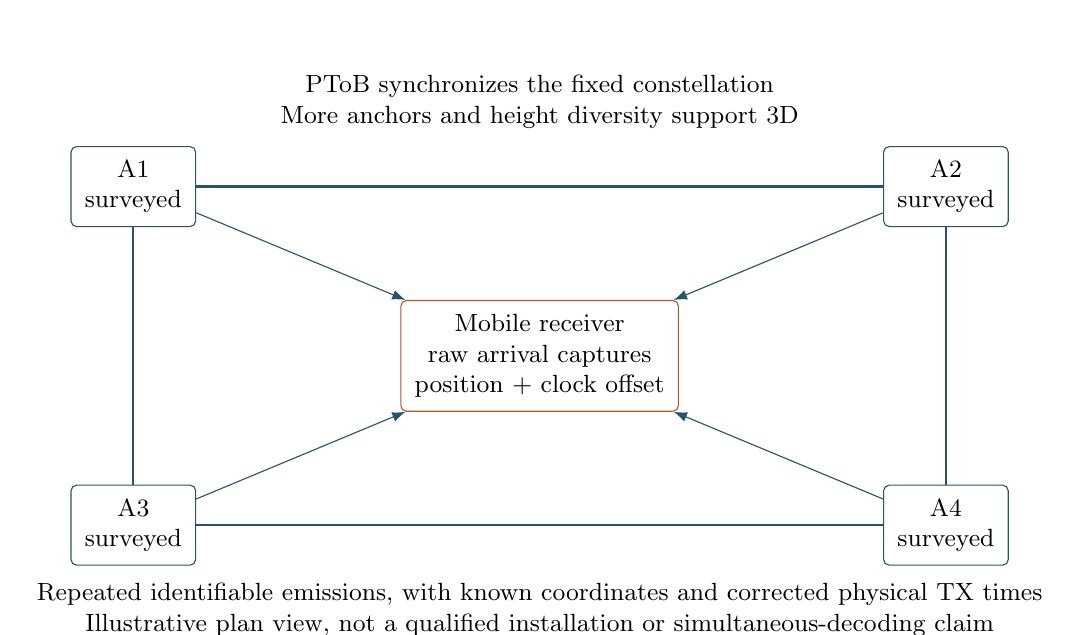
\begin{tikzpicture}[>=Latex,scale=.86,anchorbox/.style={draw=studyblue,fill=white,rounded corners=2pt,font=\small,align=center,inner sep=5pt}]
\draw[studyblue,thick](0,0) rectangle (12,5);
\node[anchorbox] (a) at (0,5) {A1\\surveyed};
\node[anchorbox] (b) at (12,5) {A2\\surveyed};
\node[anchorbox] (c) at (0,0) {A3\\surveyed};
\node[anchorbox] (d) at (12,0) {A4\\surveyed};
\node[anchorbox,draw=studyorange] (r) at (6,2.5) {Mobile receiver\\raw arrival captures\\position + clock offset};
\draw[->,studyblue](a)--(r);\draw[->,studyblue](b)--(r);\draw[->,studyblue](c)--(r);\draw[->,studyblue](d)--(r);
\node[font=\small,align=center] at (6,6.25) {PToB synchronizes the fixed constellation\\More anchors and height diversity support 3D};
\node[font=\small,align=center] at (6,-1.25) {Repeated identifiable emissions, with known coordinates and corrected physical TX times\\Illustrative plan view, not a qualified installation or simultaneous-decoding claim};
\end{tikzpicture}
\caption{Proposed local navigation constellation. Fixed beacons repeatedly transmit; many mobile receivers may listen without a per-receiver ranging exchange. The arrows represent distinct observations, not guaranteed simultaneous RF reception.}\label{fig:room}
\end{figure}

A GNSS receiver derives pseudoranges from distinguishable satellite signals and solves for position and receiver time offset using known satellite states and corrections \cite{esacode}. For PToB-IPS, fixed surveyed antenna coordinates replace satellite ephemerides; the room's shared PToB time coordinate replaces the satellite system time. Earth-orbit and atmospheric models are unnecessary at this scale, while indoor detector delay, multipath, clock-transfer error and poor vertical geometry become major concerns. UTC is optional for local positioning: a common site epoch and identified clock relationship suffice.

The analogy has a physical boundary. GNSS receivers track signal codes and their delays; advertising the current clock value alone is not a code-delay measurement. GNSS signal separation also relies on radio/baseband processing \cite{esareceiver}. A conventional BLE packet receiver is not thereby a multi-signal GNSS correlator. The first proposed adaptation preserves BLE packet reception and supplies physical TX/RX event timestamps, surveyed coordinates and clock corrections. A later PHY/baseband extension could approach the simultaneous-signal model more closely.

This distinction leaves a useful opportunity. A small number of fixed, powered beacons can spend time learning their clocks and delays, while each mobile receiver performs a compact navigation solve. The infrastructure broadcast workload can serve many listeners. The research objective is to obtain useful coarse positions from that inexpensive shared infrastructure, then determine which refinements genuinely buy additional spatial accuracy and update rate.

\section{Pseudorange measurements, clock offset and identifiability}\label{sec:model}
\subsection{What the receiver actually measures}
Let $a_i$ be surveyed beacon $i$'s antenna coordinate, $T_{ik}$ the true transmit event time on the site coordinate, and $t_{ik}$ its receive event time. For an initially stationary receiver at $p$, define $r_i=\|p-a_i\|$ and nominal propagation $t_{ik}=T_{ik}+r_i/c$, with $c=299\,792\,458\,\mathrm{m/s}$. The beacon reports
\begin{equation}
 \hat T_{ik}=T_{ik}+\alpha_i(T_{ik})+d_i^{\rm TX}+\epsilon_{ik}^{\rm TX},
\end{equation}
where $\alpha_i$ is its residual clock-map error and $d_i^{\rm TX}$ an uncorrected endpoint delay. The receiver retains a raw counter converted to nominal seconds,
\begin{equation}
 s(q_{ik})=t_{ik}+b(t_{ik})+d_i^{\rm RX}+\epsilon_{ik}^{\rm RX}.
\end{equation}
The receive delay can depend on channel, PHY, signal level and packet class; it need not be one common constant. Combining the records gives the measured pseudorange
\begin{equation}
 z_{ik}=c\{s(q_{ik})-\hat T_{ik}\}
 =r_i+B(t_{ik})-c\alpha_i+c\Delta d_i+m_{ik}+\nu_{ik},\label{eq:pseudo}
\end{equation}
where $B=cb$, $\Delta d_i=d_i^{\rm RX}-d_i^{\rm TX}$ and $m_{ik}$ is excess-path range bias. Coordinates, transmit convention and corrections must refer to the same antenna/event definition. Equation~\ref{eq:pseudo} is the proposed observable, not a measurement already exported by every PToB target.

\subsection{Averaging clock values is not a position solution}
After applicable corrections, a fixed-height receiver can solve for $(x,y,B)$; a 3D receiver solves for $(x,y,z,B)$. At least three independent observations in the former case or four in the latter are necessary local counts, with full-rank geometry and ambiguity checks still required. More beacons add redundancy; they do not automatically supply independent errors. A weighted nonlinear least-squares formulation is
\begin{equation}
 (\hat p,\hat B)=\arg\min_{p,B}\,[z-h(p,B)]^{\mathsf T}\Sigma^{-1}[z-h(p,B)],
 \qquad h_i(p,B)=\|p-a_i\|+B.\label{eq:wls}
\end{equation}
Linearization uses rows $G_i=[(p-a_i)^{\mathsf T}/r_i,\,1]$ and an observation covariance $\Sigma$ in squared range units. For a full-rank local model,
\begin{equation}
 P=(G^{\mathsf T}\Sigma^{-1}G)^{-1}.\label{eq:cov}
\end{equation}
This covariance assumes the stated stochastic model, calibrated biases and the correct solution branch; it is not a physical accuracy certificate. Arithmetic averaging of timestamps discards the range geometry and cannot replace the solve.

If all residual anchor errors are free unknowns at one epoch, $n$ measurements contain position, receiver clock and $n$ anchor offsets: the geometry is underdetermined. Stable, mutually calibrated anchor clocks or justified dynamic constraints are essential. A shared anchor-clock offset is absorbed into $B$; individual beacon offsets can imitate changes in position. Clock agreement with UTC is therefore a different requirement from differential anchor timing.

\subsection{Preserve propagation information instead of disciplining it away}
A one-way clock servo that assumes a link delay may absorb real propagation into the receiver clock map. Applying that same map to its training events can remove or bias the desired range information. The proposed receiver therefore saves native RX latches before navigation/discipline updates and estimates its own clock offset and rate jointly with position. It does not declare independently known receive time merely because it follows one of the ranging beacons. If a pre-existing clock map is used, its assumed path delay and correlation with the measurements remain explicit.

Likewise, synchronizing fixed anchors over BLE requires a known-delay model or additional constraints. Their surveyed separation supplies a nominal line-of-sight propagation correction; unknown excess path and hardware delay remain. Reciprocal calibration exchanges or an independently measured reference can constrain clock/delay ambiguity, subject to asymmetry and transfer uncertainty. Averaging cannot by itself identify an unknown constant path delay.

\section{All beacons active: observation epochs before overlapping signals}\label{sec:multiple}
\subsection{A first architecture for one ordinary radio}
The core proposal is to align the beacons' physical periodic-advertising schedules to a shared PToB epoch, then assign distinct event offsets and coordinated repetition rates. A receiver maintains multiple logical train synchronizations and tunes its one radio to each train in its reserved time slot. Several trains are therefore tracked concurrently while their RF receptions are separated in time. Each event retains its individual transmit timestamp; motion and receiver clock evolution across the observation sequence remain modeled.

Periodic advertising supplies repeated events and channel-selection information; its fixed scheduling and access-address semantics are documented separately from any positioning extension \cite{blecore,silabs}. Different packet identities or Access Addresses do not create orthogonal ranging waveforms. Overlapping packets on the same channel can collide or produce capture/selection bias; a single narrowband receive chain cannot listen to several RF channels at once. Simultaneously enabling all periodic advertisers is not sufficient to solve those problems. Multiple-train limits and scheduler/controller ownership must be established on each target.

\subsection{Align periodic timers, offsets and different beacon rates}\label{sec:multirate}
Let the shared base period be $P_0$, with epoch $T_0$. Assign beacon $i$ an integer period multiplier $m_i$, frame phase $r_i\in\{0,\ldots,m_i-1\}$ and event offset $o_i$. Its requested periodic-advertising anchors are
\begin{equation}
 S_{ik}=T_0+(r_i+k m_i)P_0+o_i,\qquad f_i=1/(m_iP_0).\label{eq:schedule}
\end{equation}
These are requested physical schedule positions, not replacements for actual RF TX timestamps. With $P_0=62.5\ms$, multipliers 1, 2 and 4 give 16, 8 and 4 Hz. Table~\ref{tab:rates} keeps four frequently heard beacons and interleaves slower auxiliary beacons. Reusing an offset is allowed only when the assigned frame phases do not overlap.

\begin{table}[ht]\centering\small
\caption{Illustrative aligned multi-rate plan. Compact-event airtime, guard and retuning assumptions are stated in the text; this is a scheduling model, not a controller implementation.}\label{tab:rates}
\begin{tabular}{@{}lrrrr@{}}\toprule
Beacon & Rate Hz & $m_i$ & Frame phase $r_i$ & Offset $o_i$, ms\\\midrule
A1&16&1&0&0\\
A2&16&1&0&1\\
A3&16&1&0&2\\
A4&16&1&0&3\\
A5&8&2&0&4\\
A6&8&2&1&4\\
A7&4&4&0&5\\
A8&4&4&2&5\\\bottomrule\end{tabular}
\end{table}

\begin{figure}[ht]\centering
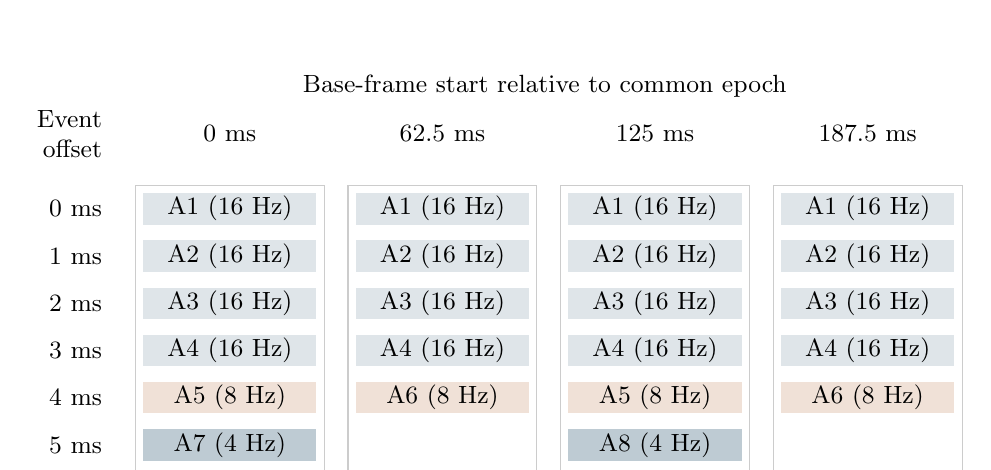
\begin{tikzpicture}[x=1cm,y=1cm,font=\small]
\foreach \x/\label in {0/0,1/62.5,2/125,3/187.5}{
 \node at (\x*2.7+1.2,.65){\label\ ms};
 \draw[gray!40](\x*2.7,0) rectangle (\x*2.7+2.4,-3.75);
}
\foreach \row/\offset in {0/0,1/1,2/2,3/3,4/4,5/5}{
 \node[anchor=east] at (-.3,-\row*.6-.3){\offset\ ms};
}
\foreach \col in {0,...,3}{
 \foreach \row in {0,...,3}{
  \fill[studyblue!15](\col*2.7+.1,-\row*.6-.1) rectangle (\col*2.7+2.3,-\row*.6-.5);
  \pgfmathtruncatemacro{\id}{\row+1}
  \node at (\col*2.7+1.2,-\row*.6-.3){A\id\ (16 Hz)};
 }
}
\foreach \col/\id in {0/5,1/6,2/5,3/6}{
 \fill[studyorange!18](\col*2.7+.1,-2.5) rectangle (\col*2.7+2.3,-2.9);
 \node at (\col*2.7+1.2,-2.7){A\id\ (8 Hz)};
}
\foreach \col/\id in {0/7,2/8}{
 \fill[studyblue!30](\col*2.7+.1,-3.1) rectangle (\col*2.7+2.3,-3.5);
 \node at (\col*2.7+1.2,-3.3){A\id\ (4 Hz)};
}
\node at (5.2,1.25){Base-frame start relative to common epoch};
\node[anchor=east,align=right] at (-.3,.65){Event\\offset};
\end{tikzpicture}
\caption{Proposed multi-train reservation grid over one 250 ms hyperperiod, not an airtime scale drawing. Four 16 Hz trains provide a frequent core; 8 Hz and 4 Hz trains reuse offsets in disjoint frames. Each receiver tunes by train and predicted RF channel within these time-separated reservations. Blank cells are idle.}\label{fig:slots}
\end{figure}

The schedule repeats after $\operatorname{lcm}(1,2,4)P_0=250\ms$. Its four base frames contain respectively six, five, six and five event windows: 22 total. The receiver keeps each train's SyncInfo, event/channel prediction and incarnation, then merges all predicted receive windows into one radio reservation calendar. Different frequencies are repetition rates here, not a claim of simultaneous reception on different RF channels. Deliberately related periods make cyclic collision checking tractable; arbitrary rates and offsets do not guarantee a feasible calendar.

If $A_i$ bounds on-air occupancy, $g_i$ is an early/late receive guard and $R_{ij}$ bounds retuning/controller transition, adjacent planned starts must satisfy
\begin{equation}
 S_j-S_i\geq A_i+g_i+g_j+R_{ij}.\label{eq:guard}
\end{equation}
For an illustrative compact future event ticket with $A_i=0.6\ms$ including on-air overhead, $g_i=g_j=0.1\ms$ and $R_{ij}=0.2\ms$, 1 ms separation is exactly filled, with no additional slack. This assumption requires a compact future record: the current roughly 190-byte timing record is not claimed to fit the 1 ms slot. Metadata and follow-up traffic require additional capacity. Actual chained PDUs, channel switching, clock-age growth and controller conflicts must be included before admission. These slots are not a PAwR timing specification or an accepted controller schedule. Check reservations over the entire hyperperiod including its wrap boundary, even if colliding trains would use different RF channels: one receive chain cannot honor both. Infeasible plans require new offsets/rates or explicit missed-observation accounting.

Physical alignment needs a measured PToB-counter-to-controller-clock relationship and bounded control over periodic-event placement. Updating a software clock map does not move an advertising timer. Ordinary host commands do not establish an arbitrary absolute event phase merely because their data includes a time. A future adapter must align or steer the controller schedule while preserving train synchronization, or announce a new activation and incarnation with sufficient discovery/reacquisition. Schedules, survey versions and channel plans need a future activation epoch, bounded guard applicability and an expiry policy. Alignment means reliably fitting known events into receive windows; it does not require all anchors' RF edges to have identical phase. Actual captured TX corrections still determine the navigation observation.

A 4 Hz auxiliary observation can approach 250 ms of age before its next update, corresponding to 1.25 m of motion at $5\,\mathrm{m/s}$. It must be fused at its own event time or propagated through a justified state model, not combined as a fresh range with the next 16 Hz core burst. Four fast beacons alone do not guarantee a 3D fix with unknown drift or poor geometry. Rate assignment must preserve the required full-rank, sufficiently fresh anchor set for the intended dynamics.

\subsection{A moving receiver needs offset, drift and motion}
For comparison, in a dense eight-beacon burst with 1 ms slot spacing, the first-to-last event span is seven milliseconds. Across that span, a residual 1 ppm receiver frequency error changes apparent range by approximately 2.099 m. At an assumed speed of $5\,\mathrm{m/s}$, position changes by 35 mm. This example shows why a stable clock map and a clock-drift state matter even when the geometric movement seems small.

A candidate model is
\begin{equation}
 z_{ik}=\|p_0+v(t_{ik}-t_0)-a_i\|+B_0+D(t_{ik}-t_0)+\xi_{ik},\label{eq:dynamic}
\end{equation}
where $D$ is receiver clock range-rate, and $\xi$ retains corrected endpoint and propagation errors. With known motion over a burst, 3D position, offset and unknown drift require at least five locally independent scalar constraints. If velocity is also free, there are eight state components before adding inertial biases; counts alone do not ensure observability. Time scheduling correlated with beacon direction can couple drift and position. Reordering slots, repeated beacons and independent rate/IMU constraints are research controls.

\subsection{True simultaneous reception is a separate future branch}
A GNSS-like overlapping-signal constellation would require separable codes, a suitable multichannel front end, or other validated multiuser processing, together with near--far control. A common clock does not grant an ordinary BLE controller those capabilities. Proprietary coded waveforms or multi-correlator receivers could be investigated on suitable radios, but may require new silicon, a different PHY and separate coexistence/regulatory/profile review. They cannot be advertised as a firmware-only capability of the installed BLE population. Scheduled epochs preserve much of the broadcast-navigation concept without making this assumption.

\section{Stable averaged clocks: the improvement and its floor}\label{sec:averaging}
\subsection{Infrastructure averaging and receiver averaging solve different problems}
Stationary powered beacons can estimate frequency and clock-map curvature over a long history, aggregate observations from multiple references and refresh calibrated corrections. An anchor ensemble may reduce independent estimation noise and identify inconsistent members. It still has a time-coordinate gauge, common-source errors and persistent endpoint delays. A software clock map disciplines numerical time; it does not establish coherent RF carriers or tune the crystal automatically.

For $M$ equally noisy clock estimates with standard deviation $\sigma$ and equal pairwise correlation $\rho$, the equal-weight mean has
\begin{equation}
 \operatorname{Var}(\bar e)=\sigma^2\{\rho+(1-\rho)/M\}.\label{eq:ensemble}
\end{equation}
For hypothetical $\sigma=30\ns$ and $M=8$, independence gives $10.607\ns$, while $\rho=0.5$ gives $22.5\ns$. A fixed unknown bias is unchanged. Optimal weighting needs the covariance and dependency structure, not just each clock's displayed RMS. Shared reference noise may cancel in some simultaneous differences or be absorbed by receiver offset, while individual anchor bias remains geometrically harmful.

Receiver averaging acts on repeated pseudoranges or a sequence of state estimates. Independent zero-mean noise can decrease as $1/\sqrt N$ for a stationary geometry. Repeated samples with lag correlation $\rho_\ell$ have
\begin{equation}
 \operatorname{Var}(\bar e)=\frac{\sigma^2}{N}
 \left[1+2\sum_{\ell=1}^{N-1}(1-\ell/N)\rho_\ell\right].\label{eq:timecorr}
\end{equation}
Fixed multipath, deterministic quantization phase, antenna delay and an unobserved clock step do not average away under the independent model. Distinct RF copies and channels can help diagnose these terms, but channel diversity alone does not prove independent unbiased measurements. Stable reference-clock frequency and stable propagation bias are both ``stable'' and have very different consequences for positioning.

\subsection{An explicit idealized room calculation}\label{sec:roomcalc}
Consider eight surveyed anchors at the corners of a $10\times8\times3\,\mathrm{m}$ rectangular room and a receiver at $(5,4,1.5)\,\mathrm{m}$. Floor-and-ceiling corners provide generous height diversity; this is an analytical geometry, not a proposed wiring or mounting prescription. All eight ranges are $\sqrt{43.25}\,\mathrm{m}$. With independent equal range variance and unknown receiver clock offset, symmetry gives horizontal dilution $H=0.744406$ and 3D dilution $P=1.719569$ from Equation~\ref{eq:cov}.

Assume, solely for sensitivity analysis, 30 ns independent zero-mean per-beacon pseudorange time noise in each epoch. The expected linearized horizontal RMS is $Hc\sigma_t/\sqrt N$. A separate hypothetical 5 ns per-anchor persistent offset, drawn independently across anchors and fixed throughout an averaging window, instead gives
\begin{equation}
 E_{H,\mathrm{model}}=Hc\sqrt{(30\ns)^2/N+(5\ns)^2}.\label{eq:floor}
\end{equation}
The expression is an ensemble stochastic model for those assumptions, not a bound for a particular set of biases. It is not derived by reinterpreting published PToB PPS RMS as ranging noise.

\begin{table}[ht]\centering\small
\caption{Analytical horizontal RMS at the room centre. Linearization, perfect survey, calibrated receive conventions and stationary geometry are assumed. No RF experiment or Monte Carlo campaign produced these values.}\label{tab:average}
\begin{tabular}{@{}rrrr@{}}\toprule
Epochs $N$ & Collection $N/16$ (s) & Independent only (m) & With 5 ns floor (m)\\\midrule
1&0.0625&6.695&6.787\\
16&1&1.674&2.012\\
256&16&0.418&1.192\\\bottomrule\end{tabular}
\end{table}

The hypothetical floor alone corresponds to 1.116 m horizontal RMS in this geometry. Thus long averaging offers a plausible coarse static-position experiment if the biases are first constrained; it is not an argument for arbitrarily accurate navigation. At $5\,\mathrm{m/s}$, a receiver travels 80 m during a 16 s collection. A drone cannot simply average those observations as a single stationary position. Long anchor-clock estimation can continue while mobile positioning uses short epochs and a dynamic filter.

\begin{figure}[ht]\centering
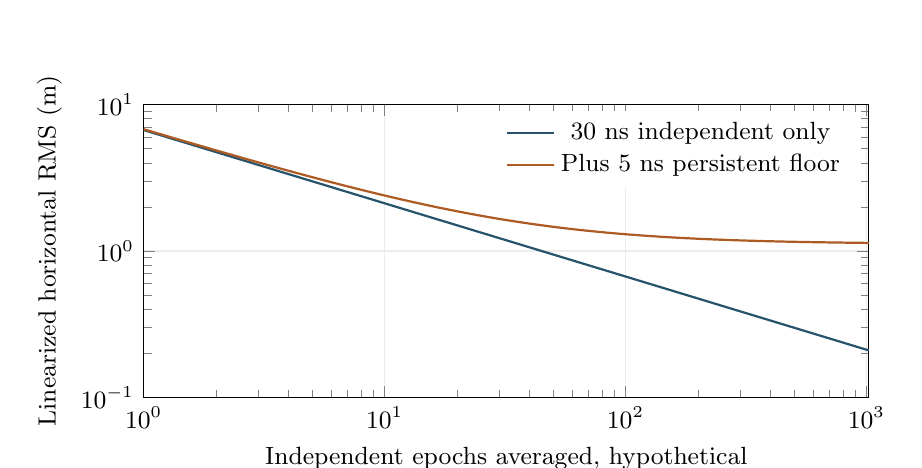
\begin{tikzpicture}
\begin{loglogaxis}[width=.89\linewidth,height=53mm,xmin=1,xmax=1024,ymin=.1,ymax=10,xlabel={Independent epochs averaged, hypothetical},ylabel={Linearized horizontal RMS (m)},grid=major,grid style={gray!15},tick label style={font=\small},label style={font=\small},legend style={font=\small,draw=none,at={(.98,.98)},anchor=north east}]
\addplot[studyblue,thick,domain=1:1024,samples=80]{6.69502114127/sqrt(x)};\addlegendentry{30 ns independent only}
\addplot[studyorange,thick,domain=1:1024,samples=80]{.223167371376*sqrt(900/x+25)};\addlegendentry{Plus 5 ns persistent floor}
\end{loglogaxis}
\end{tikzpicture}
\caption{Analytical sensitivity, not achieved IPS accuracy. Temporal correlation, nonlinear ambiguity, receiver motion, survey error and NLOS are absent. The noise-only curve continues downward because that assumption was built into it.}
\end{figure}

\section{What higher-MHz clocks can and cannot buy}\label{sec:finer}
\subsection{Capture resolution, clock stability and RF information are distinct}
For a capture clock $f$, the nominal tick is $q=1/f$. A uniformly distributed quantization error has standard deviation $q/\sqrt{12}$. If TX and RX stamps have independent equal quantization errors, their one-way difference contributes range standard deviation
\begin{equation}
 \sigma_{r,q}=c\sqrt{q_{\rm TX}^2+q_{\rm RX}^2}/\sqrt{12}
             =\frac{c}{f\sqrt6}\quad(q_{\rm TX}=q_{\rm RX}=1/f).\label{eq:quant}
\end{equation}
This is only a quantization component, not total error or an independence guarantee. Rounding bias and locked sampling phases can invalidate the uniform model. Known phase diversity may support sub-tick statistical estimation under a validated detector model; adding random delays without measuring their actual RF events creates additional uncertainty instead.

\begin{table}[ht]\centering\small
\caption{Hypothetical equal TX/RX capture grids. Higher frequencies do not assert a supported peripheral mode. No synchronization, detector, multipath or survey error is included.}\label{tab:timer}
\begin{tabular}{@{}rrrr@{}}\toprule
Capture MHz & Tick ns & One-tick range m & Two-stamp $\sigma_{r,q}$ m\\\midrule
16&62.5&18.737&7.649\\
80&12.5&3.747&1.530\\
160&6.25&1.874&0.765\\
240&4.166667&1.249&0.510\\
1000&1&0.300&0.122\\\bottomrule\end{tabular}
\end{table}

Increasing a physically available capture clock can therefore help a coarse IPS substantially if quantization is important. In the optimistic independent-quantizer model, an 80 MHz pair is already associated with a 1.530 m range-noise component before averaging and geometric dilution. Finer clocks, multiphase interpolation or low-cost time-to-digital peripherals could reduce that component further. A 1 GHz row is an effective-resolution thought experiment, not an existing PToB MCU requirement or a supported clock-setting suggestion.

Nordic documents the nRF52840 TIMER base at 16 MHz divided by its prescaler \cite{nordic}. Espressif documents that ESP32-S3 MCPWM capture follows its APB clock rather than accepting an arbitrary requested resolution \cite{espressif}; the existing PToB fine-capture study uses 80 MHz raw capture and a delivered coordinate rounded to 50 ns \cite{fine}. Changing a CPU frequency, timestamp integer unit or advertised precision field does not make that path finer. IPS research should retain the native capture and fractional-map information before delivery rounding, while accounting for the actual synchronizers and detector grid.

A finer timer timestamps the radio detector's output more finely. It does not make a narrowband packet into a broadband delay measurement or separate direct path from a nearby reflection. NIST's indoor propagation work illustrates why multipath and obstructed direct paths remain localization limits even with dedicated ranging waveforms \cite{nistindoor}. RF delay estimation, SNR, signal level, packet structure, channel dependence and analog group delay must be characterized alongside the counter.

\subsection{Required differential time follows the desired spatial task}
One-way propagation converts 10 ns to 2.998 m and 1 ns to 0.300 m. Allocating 1 m to a range-error component permits 3.336 ns; 0.10 m permits 333.564 ps. Actual position error also depends on geometry. Coarse room/zone inference may tolerate a larger budget than local collision avoidance, but can still fail near walls or between adjacent rooms. A task requirement must be converted into a differential timing, endpoint and propagation budget before choosing clock frequency.

If an unknown anchor-specific bias has a 10 ns scale, raising capture from 80 to 240 MHz cannot by itself meet a 0.3 m position target. Conversely, once that bias is calibrated below a few nanoseconds, a finer capture path and independent short-window samples become a more credible investment. The development priority is joint: better RF event semantics, bias calibration, stable relative clocks, sufficient capture resolution and useful geometry.

\section{Protocol adaptation: a proposed PToB-IPS extension}\label{sec:protocol}
\subsection{Preserve the timing network; add a navigation observation service}
PToB-IPS is a paper-level research label, not a new assigned protocol identifier or frozen wire layout. The aligned periodic-timer, multi-rate offset plan in Section~\ref{sec:multirate} is its proposed access architecture. Existing GM/RC authority, authentication, counter ownership, source expiry and ordinary timing service retain their own contracts. An observation-capable receiver may listen to several beacon identities for navigation without making them simultaneous timing parents or importing their source authority. Current single-parent control and a future multi-anchor measurement collector are different mechanisms.

The proposed extension separates infrequent beacon/schedule metadata from compact physical-event tickets and authenticated follow-up corrections. The schedule metadata includes base epoch/period, per-train multiplier, frame phase, offset, RF discovery/channel information, receive-window budget, activation version and expiry. It reuses PToB's principle of binding a later timestamp correction to an exact earlier event \cite{v14paper}. A scheduled launch time remains an estimate until the actual RF event and endpoint convention are established. Some targets have defined hardware radio events; others currently provide empirical receive markers and estimated TX. Those capability classes must be visible to the solver.

\begin{table}[ht]\centering\small
\caption{Proposed logical information groups. Byte encodings, fragmentation, capacity and authentication policy require a later reviewed engineering specification.}\label{tab:contract}
\begin{tabular}{@{}L{31mm}L{114mm}@{}}\toprule
Information group & Meaning needed for a ranging observation\\\midrule
Surveyed beacon &Anchor/site/frame identity, coordinates and units, antenna reference point, survey revision, uncertainty and movement invalidation.\\\addlinespace
Clock model &Site epoch, clock incarnation, map generation, reference epoch, offset/rate corrections, age/expiry, calibrated versus unknown error terms and shared-source correlation group.\\\addlinespace
Physical event &Anchor boot/train, publication and physical-copy identity, event counter, PHY/channel/packet class, endpoint convention and raw TX capture or declared estimate.\\\addlinespace
Follow-up &Corrected TX time for the exact prior event, supporting map/calibration revisions, validity, uncertainty scope and immutable association.\\\addlinespace
Receiver record &Raw RX latch/incarnation, nominal frequency model, receive convention, signal/channel diagnostics, unmatched/ambiguous status and correction arrival time.\\\addlinespace
Navigation result &State epoch/frame, position/velocity, clock offset/drift, covariance applicability, anchor set, geometry/health, age, latency and reject/degrade reason.\\\bottomrule
\end{tabular}
\end{table}

\subsection{Keep causality and unavailable observations visible}
A receiver buffers each raw event until it can match the authenticated correction and required metadata. Corrections may arrive in a later broadcast; the output latency includes that wait. Use only source and map information permitted by the declared causal decision time for an online score. If later information supports retrospective reprocessing, label that result separately. Repetitions of the same event or correction are redundancy, not additional independent ranges. Missing, collided, ambiguous, expired and source-invalid events remain explicit denominator classes.

The anchor's corrected TX time must use a map valid for the physical event and preserve its original source validity. Reset, counter wrap ambiguity, antenna relocation, PHY convention changes or retired survey/calibration revisions fence affected observations. An integer epoch or fine timestamp width cannot repair a wrong physical copy association.

\subsection{Calibrate the constellation before solving the mobile unknown}
A practical calibration sequence would survey anchor antenna coordinates; measure reference-to-anchor path and relative clock behavior; establish TX/RX endpoint delay by target, PHY, channel, orientation and signal regime; freeze corrections on training observations; then validate at independent held-out positions and boots. Reference receivers at surveyed positions can supply differential correction observations, provided their own path/detector uncertainty and correlations are carried forward. Multi-anchor reciprocal measurements can add constraints without proving symmetric propagation automatically.

Averaged anchor clocks may be refreshed continuously, but calibration applicability and expiry must remain bounded. Online self-calibration from mobile trajectories is a later joint estimation problem with clock, position and delay gauge freedoms; it cannot silently replace an independent reference. A small fitted residual at the training points is not held-out spatial accuracy.

\section{An adoption path across commodity MCU capability classes}\label{sec:adoption}
\subsection{A large ecosystem, with an unknown compatible subset}
The ambition is to make indoor navigation accessible across a very large existing MCU ecosystem. A Bluetooth SIG-hosted 2026 industry article reports more than five billion Bluetooth devices shipped annually \cite{market}. Shipment volume is not an installed-MCU count, a PToB-compatible count or a count of accessible radio timestamps. The claim here is potential reach through an inexpensive common design, not firmware upgradeability of billions of existing units.

\begin{table}[ht]\centering\small
\caption{Proposed capability classes; a device must demonstrate its class. Hardware generation or CPU MHz alone is insufficient.}\label{tab:classes}
\begin{tabular}{@{}L{33mm}L{57mm}L{55mm}@{}}\toprule
Class & Possible contribution & Main adoption boundary\\\midrule
Packet-only legacy &Decode beacon identity/metadata; provide discovery or a host for an external observation source. &Host packet-arrival timestamps do not establish propagation ranging.\\\addlinespace
Event-capture MCU &Native RX capture, defined or calibrated TX event, raw counter and multi-beacon collection; candidate coarse pseudoranges. &Controller access, capture grid, closed firmware, buffer limits and detector calibration.\\\addlinespace
Refined timing target &Higher-rate capture or measured interpolation, improved TX/RX semantics and tighter calibrated relative clocks. &Actual peripheral capability, phase noise, power and RF delay floor.\\\addlinespace
Phase-capable future radio &Packet timing plus phase/frequency observations or qualified simultaneous signal separation. &New baseband features, oscillator/antenna calibration, ambiguity resolution and compatibility.\\\bottomrule
\end{tabular}
\end{table}

The most attractive first cohort is MCU radios already exposing useful hardware events and modifiable controller integration. Portability work would standardize observation semantics and capability reporting before optimizing a solver. A compact least-squares state has modest arithmetic demands; obtaining honest radio timestamps and maintaining multiple observation trains may be the larger obstacles. A secure field update path, spare timers, memory, energy and access to the relevant firmware cannot be assumed for deployed products.

\subsection{Economic leverage comes from passive listeners and reuse}
A surveyed broadcast constellation can serve many receivers without requiring a two-way exchange for each tag and anchor. Its baseline navigation broadcast load scales with beacon activity rather than listener count; enrollment, telemetry, interference and optional feedback can still grow with the fleet. Repurposed powered infrastructure may reduce new hardware, but only when placement, survey, firmware ownership and RF capture are adequate.

The budget hypothesis is lower incremental radio and integration cost for a coarse service by reusing BLE MCU hardware. Compare total cost for the same accepted accuracy, availability, latency and coverage, including survey, commissioning, recalibration, maintenance and power. This paper uses no product-price quotation or measured saving. If calibration and maintenance overwhelm radio reuse, the budget argument fails. Improving a passive fleet's position service while keeping compatible legacy listeners functional is a protocol goal, not a demonstrated migration.

\section{A roadmap from coarse IPS to robotic and drone PNT}\label{sec:roadmap}
\subsection{Stage 1: position from surveyed timing beacons}
Start with stationary or slowly moving receivers and a declared height constraint. Collect actual radio events from more than the minimum beacon set, preserve native counters, freeze all delay corrections, and compare a GNSS-like solve against surveyed truth. The first question is whether calibrated pseudorange changes follow known changes in geometric distance. If they do not, internal clock RMS and solver convergence cannot establish IPS feasibility. A useful first objective is coarse spatial discrimination with complete availability accounting, not an inherited sub-metre target.

A proposed pilot could use six to eight anchors in a measured room, hold out entire grid locations from calibration and test multiple boards and boots. Candidate research gates might be horizontal P95 at most 5 m, at least 95\% valid position availability and explicitly bounded reporting latency for static or low-dynamic trials. These are study-design examples, not claims of usefulness in every room. Report false room assignment near boundaries, persistent bias and wrong-but-plausible outputs, rather than accepting a low average over favourable locations.

\subsection{Stage 2: shorter epochs and finer physical timing}
Develop actual TX capture/association where missing, preserve fractional native observations, compare validated capture grids, characterize channel/signal-level delay, and measure differential anchor timing independently. Use slot ordering controls to separate position from clock drift. Improve anchor placement and height diversity. An elevated receiver with ceiling-only anchors may have ambiguous or weak vertical information; at the symmetric centre in the corner geometry, retaining only the four ceiling anchors makes height and clock offset locally inseparable. General coplanar layouts need their own rank and ambiguity analysis.

Only then ask whether short-latency metre-scale fixes can be maintained under motion, occlusion and coexistence. A faster capture clock should be judged by held-out spatial improvement under the same RF conditions and averaging latency. A reported precision improvement that depends on extending the window beyond the motion budget does not pass this stage.

\subsection{Stage 3: dynamic navigation and additional BLE observables}
A drone or robot combines beacon observations with a motion model and onboard inertial/odometric information while retaining beacon pseudoranges as the central external positioning input. This is a way to propagate between fixes and handle short bursts, not a substitute for range observability. Clock offset/drift, antenna lever arm, attitude-dependent delay and observation age enter the estimator. Rapid yaw, metal shelving, rotor/electrical noise, body blockage and source transitions require separate tests. Coarse position is not an obstacle-avoidance or flight-control guarantee.

Future phase/frequency measurements could complement packet timing. A coherent one-way phase difference has ideal dependence $\Delta\phi=2\pi\Delta f\,r/c$ modulo phase ambiguity, but unknown transmit phase and channel/oscillator resets obstruct that interpretation on ordinary radios. Existing Bluetooth Channel Sounding explicitly provides phase-based ranging and round-trip timing on supporting controllers \cite{channelsounding}; that is a hardware/protocol feature boundary, not a capability inherited by every legacy BLE device. Any proposed packet/phase hybrid must retain ambiguity and multipath models and distinguish software time-map agreement from RF coherence.

\subsection{UWB as an intermediate option, not the baseline}
A UWB subsystem can provide an optional independent ranging reference or an intermediate higher-accuracy service while the BLE beacon approach matures. It can help evaluate the shared navigation interface and difficult timing budgets. This manuscript does not design that integration or presume universal UWB cost or deployment figures. The central research path is to extract useful positioning from commodity BLE timing hardware and identify the specific inexpensive refinements needed to go further.

\section{Validation that can reject the hypothesis}\label{sec:validation}
\begin{table}[ht]\centering\small
\caption{Proposed evidence gates. No experiment in this table has been performed for this paper.}\label{tab:gates}
\begin{tabular}{@{}L{29mm}L{67mm}L{49mm}@{}}\toprule
Question & Required comparison & Failure kept visible\\\midrule
Does delay encode range? &Known distance changes with frozen TX/RX conventions, independent timing/position truth, repeated channels and signal levels. &No geometric response, detector changes, tails and unavailable physical events.\\\addlinespace
Do stable clocks help? &Independent relative-anchor clock observation; separate common and individual terms; averaging versus correlation and bias. &Bias floor, shared errors and an offset fitted using evaluation positions.\\\addlinespace
Can one receiver collect enough? &Actual multi-train/controller capability; prespecified epochs; collisions, slot guards, retuning and follow-up latency. &Missed anchors, ambiguous joins, near--far selection and partial epochs.\\\addlinespace
Does MHz improve IPS? &Same target semantics, waveform, geometry and latency; raw grid/interpolation and full spatial error compared. &Better tick size without better held-out range or position.\\\addlinespace
Can motion be tracked? &Clock/motion-state ablation, independent trajectory truth, multiple speeds and slot orders; no stationary averaging of moving ranges. &Clock/position coupling, biased tracking, outages and latency excursions.\\\addlinespace
Does reuse save cost? &Equal accepted service versus a stated baseline; engineering, survey, recalibration, power and replacement counted. &Unusable legacy paths, coverage exclusions and maintenance costs.\\\bottomrule
\end{tabular}
\end{table}

Freeze source revisions, board/antenna profile, survey/calibration versions, radio settings, epoch schedule and eligibility rules before held-out evaluation. Separate calibration points, positions, devices and days from those used to score transfer. Retain raw event identity and actual correction availability so offline truth does not train an earlier online solution.

For each nominal epoch report the complete counts of physical observations, decoded events, exact TX/RX joins, reference-valid observations, full-rank solves, delivered states and truth-scorable outputs. A missing fix is unavailable, not zero error. Rejects selected by a quality rule remain in availability accounting; large errors must not be relabelled invalid after seeing truth. Report horizontal and vertical bias, RMS, P95/P99, maximum, latency, source age, longest outage, and room/zone confusion. State whether error is absolute in the surveyed frame or aligned retrospectively. Count wrong but valid-looking fixes as errors.

Averaging experiments must plot error versus observation count \emph{and elapsed time}, quantify temporal/cross-anchor dependence and retain all tails. Use blocks or repeated independent trials when constructing uncertainty statements; thousands of adjacent samples are not automatically independent. Test loss of individual anchors, source changes, partitions, moving or mis-surveyed anchors and expired corrections. Authenticated data identifies a sender; it does not certify its location or prevent propagation-delay manipulation.

\section{What exists today and what remains theoretical}\label{sec:evidence}
The latest discussed public timing collection is dated 24 October 2026. Its W12 two-window relative-PPS population has 522 eligible of 600 logged records, 60.328 ns RMS including bias and a 180 ns maximum. Its complete second 300-second window, a subset, has 38.312 ns RMS and a 121 ns maximum. The 78 source-unavailable records remain. The downstream population has 451 eligible of 600, 61.922 ns RMS and a 211 ns maximum; selected received-path TX has 58 eligible of 120 and a 226 ns maximum \cite{w12}.

The separate 22 October N30 experiment has 657 eligible of 660, 166.590 ns RMS and a 1591 ns tail; a later distinct 48-of-64 transfer has 150.954 ns RMS \cite{fine}. Its empirical receive-marker convention, estimated TX and the different hardware/profile prevent interpreting it as a calibrated ranging result. These populations are neither pooled nor used as the 30 ns random-noise input in the room example.

Those results establish motivation for better relative-time infrastructure under their recorded scope. They do not measure per-beacon pseudorange noise, differential anchor RF timing, position accuracy, calibrated absolute UTC or compatibility with GNSS time transfer. The IPS solver, multi-beacon collector, compact protocol records, fine-grid comparisons and simultaneous-signal branch proposed here have not been implemented or qualified. The analytical examples are first-order sensitivity calculations with ideal survey and stated error assumptions. They are reproducible and intentionally falsifiable, not a simulator acceptance claim or a prediction that current firmware can locate a drone.

\section{Conclusion}
A constellation of surveyed PToB beacons is a credible research direction for budget indoor positioning: repeatedly transmit identifiable physical events, distribute corrected transmit time and coordinates, and let many receivers solve for their position and clock state. Stable averaged infrastructure clocks are useful because they reduce a difficult part of the measurement problem; their value emerges only when propagation and radio endpoint delays remain observable and calibrated.

The proposed first step is coarse positioning from aligned periodic-advertising timers, assigned offsets and coordinated rates that let one capable MCU receiver track multiple beacon trains in distinct time slots. Finer capture grids, improved TX/RX event semantics, bias control and later phase or multiuser radio features form a quantitative refinement path. Broad deployment is an adoption ambition conditioned on actual device capability. The research succeeds if held-out geometric positioning improves at useful latency and total cost; it fails if averaging only smooths an unidentified bias or if the radio cannot expose the required observations.

\appendix
\section{Offline analytical supplement and edition identity}
The self-contained source is \path{papers/indoor-ips/main.tex}; original vector figures and bibliography are embedded. The matching review PDF is \path{papers/indoor-ips/main.pdf}. The dated receipt \path{papers/editions/indoor-ips-2026-10-26.json} binds source, PDF, executable analysis, analytical JSON and existing public evidence inputs.
\begin{quote}\small\ttfamily
mkdir -p artifacts/indoor-ips-build\\
tectonic --outdir artifacts/indoor-ips-build papers/indoor-ips/main.tex\\
python3 tools/verify\_indoor\_ips\_paper.py
\end{quote}
Tectonic may fetch public typesetting dependencies on first use. Standard-library Python checks unit conversions, clock averaging/correlation, quantization, room covariance and geometry rank, noiseless nonlinear pseudorange recovery, clock-offset gauge, a persistent-bias counterexample, burst/motion arithmetic and edition identities. The supplement \path{papers/indoor-ips/analysis.json} is explicitly analytical model output under CC BY 4.0. It is not hardware evidence. Existing relative-clock statistics remain in their original collections; their verifiers can be run separately.

The primary-source review was performed on 26 October 2026 and is not a complete literature or normative conformance audit. Historical evidence remains bounded by its edition, profile and denominators. The earlier sensor-fusion paper and its receipt remain unchanged. This new draft awaits author review before any main-branch commitment or public publication. No firmware modification, hardware action, standards proposal submission or publication promotion accompanies its preparation.

\begin{thebibliography}{14}\small\setlength{\itemsep}{4pt}
\bibitem{viability} J. Yantis. \emph{PToB Viability: Rooted BLE Timing Meshes for Heterogeneous Edge Networks}. Research draft, 16 October 2026. \url{https://github.com/yantisj2/PToB/blob/main/papers/ptob-viability-preprint.tex}.
\bibitem{implementation} J. Yantis. \emph{Low-Level Timing on ESP32-S3: Event Capture, Clock Bridges, and Causal Validation}. Research draft, 24 October 2026. \url{https://github.com/yantisj2/PToB/blob/main/papers/ptob-esp32s3-low-level-timing.tex}.
\bibitem{esacode} J. Sanz Subirana, J. M. Juan Zornoza and M. Hern\'andez-Pajares. \emph{Code Based Positioning (SPS)}. ESA Navipedia, 2011; accessed 26 October 2026. \url{https://gssc.esa.int/navipedia/index.php/Code_Based_Positioning_(SPS)}.
\bibitem{esareceiver} ESA Navipedia. \emph{Generic Receiver Description}. Accessed 26 October 2026. \url{https://gssc.esa.int/navipedia/index.php/Generic_Receiver_Description}.
\bibitem{blecore} Bluetooth SIG. \emph{Core Specification v6.3, Vol. 6, Part B: Link Layer Specification}. Selected access-address and periodic-advertising clauses inspected, accessed 26 October 2026; no conformance audit. \url{https://www.bluetooth.com/wp-content/uploads/Files/Specification/HTML/Core_v6.3/out/en/low-energy-controller/link-layer-specification.html}.
\bibitem{silabs} Silicon Labs. \emph{Periodic Advertising}. Official implementation documentation, accessed 26 October 2026; no general phone/stack capability inferred. \url{https://docs.silabs.com/bluetooth/latest/bluetooth-fundamentals-advertising-scanning/periodic-advertising}.
\bibitem{nordic} Nordic Semiconductor. \emph{nRF52840 Product Specification: TIMER---Timer/counter}. Official peripheral documentation, accessed 26 October 2026. \url{https://docs.nordicsemi.com/r/bundle/ps_nrf52840/page/timer.html}.
\bibitem{espressif} Espressif. \emph{ESP-IDF v5.5.5 Programming Guide: MCPWM, ESP32-S3}. Capture timer and resolution documentation, accessed 26 October 2026. \url{https://docs.espressif.com/projects/esp-idf/en/v5.5.5/esp32s3/api-reference/peripherals/mcpwm.html}.
\bibitem{fine} J. Yantis. \emph{ESP32-S3 empirical fine-capture follow-up}. Public selected evidence, 22 October 2026. \url{https://github.com/yantisj2/PToB/tree/main/evidence/s3/2026-10-22-fine}.
\bibitem{nistindoor} NIST. \emph{Indoor Localization}. Archived primary project summary, accessed 26 October 2026. \url{https://www.nist.gov/ctl/smart-connected-systems-division/indoor-localization}.
\bibitem{v14paper} J. Yantis. \emph{Passive Precision Time over BLE: V14 Boundary Clocks, Causal Timestamping, and Prospective One-Relay Validation}. Research draft, 12 October 2026; historical protocol edition. \url{https://github.com/yantisj2/PToB/blob/main/papers/ptob-v14-preprint.tex}.
\bibitem{market} P. Karlsson. \emph{Bluetooth technology for industrial monitoring, tracking, and predictive maintenance}. Bluetooth SIG-hosted industry article, 9 March 2026; shipment statement attributed to ABI Research, accessed 26 October 2026. \url{https://www.bluetooth.com/blog/bluetooth-technology-for-industrial-monitoring-tracking-and-predictive-maintenance/}.
\bibitem{channelsounding} Bluetooth SIG. \emph{Bluetooth Channel Sounding: A Technical Overview}. Official explanatory document, accessed 26 October 2026; mechanisms and controller-support boundary only. \url{https://www.bluetooth.com/channel-sounding-tech-overview/}.
\bibitem{w12} J. Yantis. \emph{W12 baseline after the T096 UTC-basis repair}. Public selected evidence, 24 October 2026. \url{https://github.com/yantisj2/PToB/tree/main/evidence/s3/2026-10-24-w12-utc-basis}. Exact cited local inputs are sealed in this paper's receipt.
\end{thebibliography}
\end{document}
